\section{Zimny start}\label{chapter:results_cold_start}

\begin{figure}[h]
    \centering
    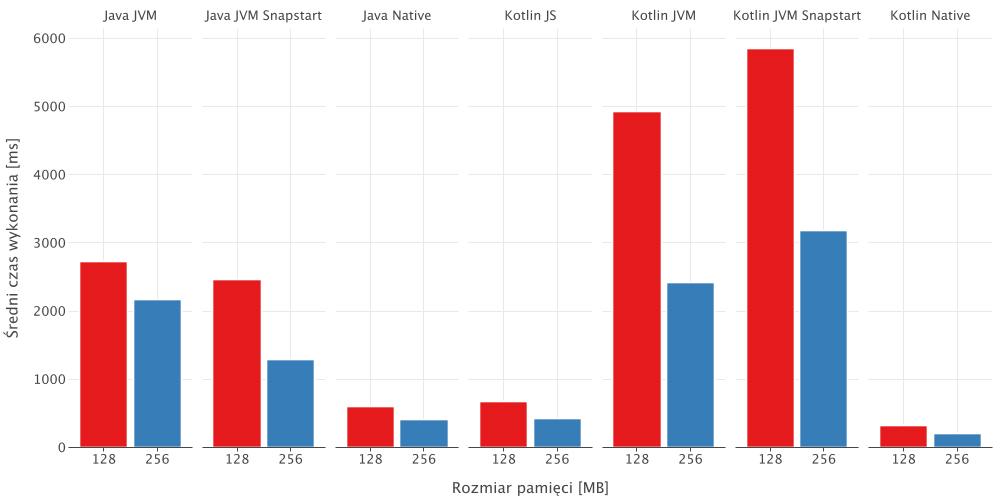
\includegraphics[width=0.95\textwidth]{charts/results/avg-cold-start-128-256.png}
    \caption{Średni czas wykonywania funkcji (zimny start) dla rozmiarów pamięci: 128 MB, 256 MB  [źródło: opracowanie własne]}
    \label{fig:avg_cold_start_128_256}
\end{figure}

\begin{figure}[h]
    \centering
    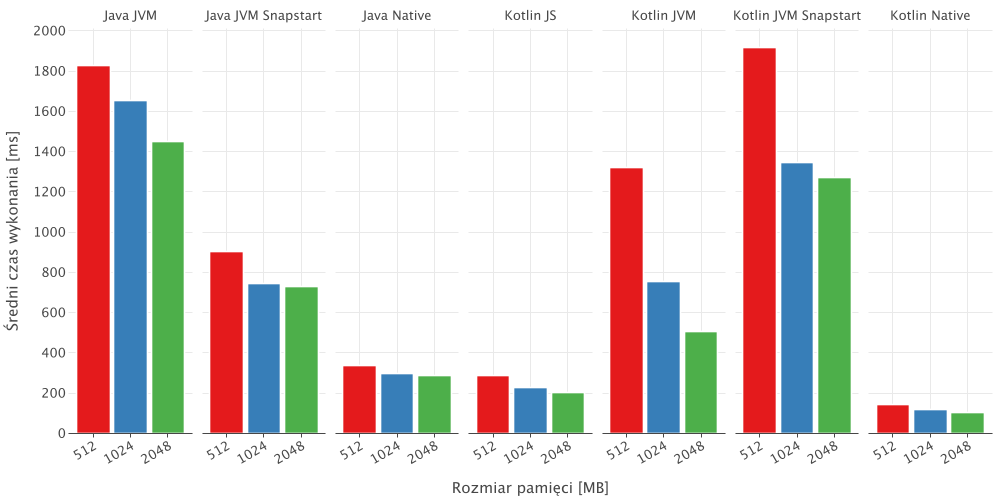
\includegraphics[width=0.95\textwidth]{charts/results/avg-cold-start-512-2048.png}
    \caption{Średni czas wykonywania funkcji (zimny start) dla rozmiarów pamięci: 512 MB, 1024 MB, 2048 MB  [źródło: opracowanie własne]}
    \label{fig:avg_cold_start_512_2045}
\end{figure}

% --- Row 1: 256 MB and 1024 MB charts ---
\begin{figure}[htbp]
    \centering % Center the minipages on the line
    \begin{minipage}[t]{0.48\textwidth} % [t] for top alignment
        \centering % Center content within this minipage
        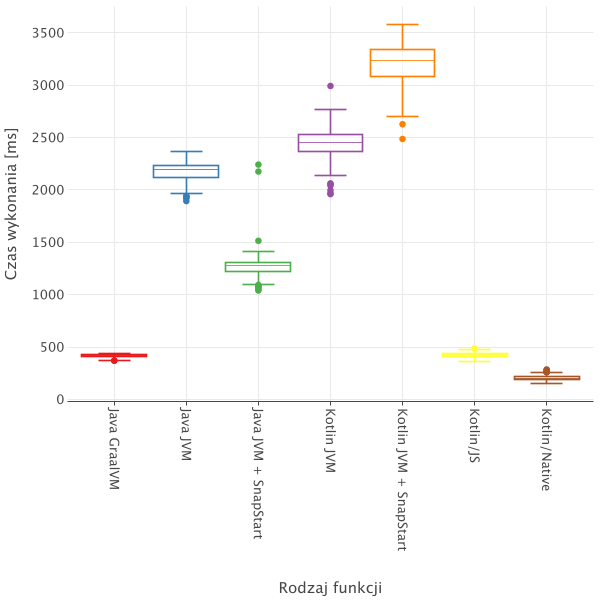
\includegraphics[width=\linewidth]{charts/results/cold-start-boxplot-256.png}
        \captionof{figure}{Czas wykonania funkcji (zimny start, 256 MB) [źródło: opracowanie własne]}
        \label{fig:cold_start_128} % Unique label for this figure
    \end{minipage}% <--- % is important
    \hfill % Space between minipages
    \begin{minipage}[t]{0.48\textwidth}
        \centering
        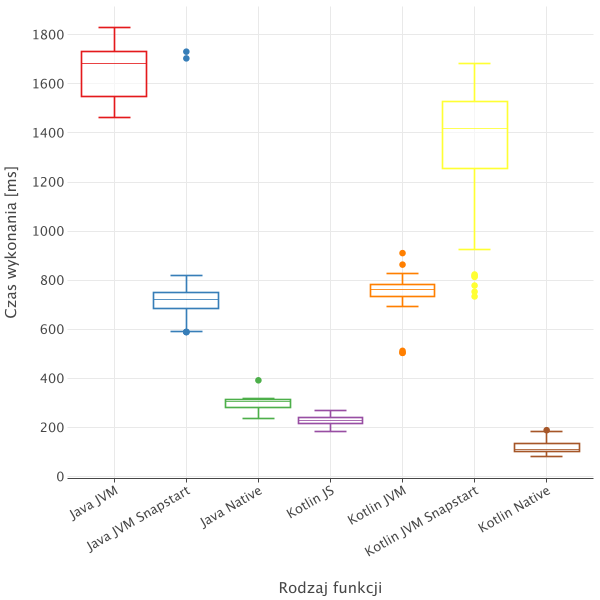
\includegraphics[width=\linewidth]{charts/results/cold-start-boxplot-1024.png}
        \captionof{figure}{Czas wykonania funkcji (zimny start, 1024 MB) [źródło: opracowanie własne]}
        \label{fig:cold_start_256} % Unique label
    \end{minipage}
    % No overall \caption for this outer figure environment, as it's just for layout.
\end{figure}

Drugim badanym kryterium jest czas działania funkcji podczas zimnych startów, które wymagają odpowiedniej inicjaliacji funkcji.
Z reguły są one dłuższe niż ciepłe starty, co może szczególnie wpłynąć na ogólną wydajność \cite{9284261}\cite{8605777}.
Średni czas działania funkcji został przedstawiony na Rysunkach \ref{fig:avg_cold_start_128_256} oraz \ref{fig:avg_cold_start_512_2045}.

Wpływ aktywacji usługi SnapStart jest różny w zależności od języka oprogramowania.
Dla Javy, usługa ta pozwoliła na poprawę czasu działania funkcji, w szczególności dla większych rozmiarów pamięci.
W przypadku języka Kotlin, jej aktywacja wpłynęła negatywnie na wydajność, wydłużając czas procesowania.
Samo użycie Kotlina (działającego w oparciu o JVM) pozwoliło na przyspieszenie obliczeń dla większych rozmiarów pamięci (512-2048 MB).

Znaczna poprawa wydajności została osiągnięte dla funkcji opartych o GraalVM oraz Kotlin/JS.
Obie metody uzyskały podobne wyniki, przy czym funkcja natywna GraalVM osiągnęła poprawę w przypadku rozmiarów pamięci 128 MB i 256 MB.
Dla wielkości 512-2048 MB, Kotlin/JS osiągnął niższe czasy działania niż funkcja GraalVM.
Niezależnie od rozmiaru pamięci najkrótszy czas działania w przypadku zimnego startu osiągnęły funkcje oparte o technologię Kotlin/Native.
Metoda ta pozwoliła także na osiągnięcie wyników o podobnej stabilności jak pozostałe funkcje, co zostało przedstawione na Rysunkach \ref{fig:warm_start_256} i \ref{fig:warm_start_1024}.
Mocno zróżnicowane wyniki zostały osiągnięte przez funkcję Kotlin z aktywowaną funkcją SnapStart.

\begin{table}[!h]
    \caption{Porównanie średnich czasów działania funkcji podczas zimnego startu względem funkcji bazowej [źródło: opracowanie własne]}
    \centering
    % Modified column definitions for left alignment
    \begin{tabular}{|>{\raggedright\arraybackslash}p{3.5cm}|>{\raggedright\arraybackslash}p{1.8cm}|>{\raggedright\arraybackslash}p{1.8cm}|>{\raggedright\arraybackslash}p{1.8cm}|>{\raggedright\arraybackslash}p{1.8cm}|>{\raggedright\arraybackslash}p{1.8cm}|}
    \hline
    % Header: First cell's \makecell changed to [l] for left alignment
    \multirow{2}{*}{\makecell[l]{\textbf{Rodzaj funkcji} \\ \scriptsize{\textit{Czas [ms] (\% różnicy)}}}} & \multicolumn{5}{c|}{\textbf{Rozmiar pamięci [MB]}} \\ % Kept multicolumn centered, change 'c' to 'l' if left-align needed
    \cline{2-6} 
    & \textbf{128} & \textbf{256} & \textbf{512} & \textbf{1024} & \textbf{2048} \\
    \hline
    Java JVM & 2726 & 2165 & 1827 & 1652 & 1450 \\
    \hline
    Java JVM +~SnapStart & 2466 \mbox{(-10\%)} & 1287 \mbox{(-41\%)} & 901 \mbox{(-51\%)} & 745 \mbox{(-55\%)} & 731 \mbox{(-50\%)} \\
    \hline
    Java GraalVM & 596 \mbox{(-78\%)} & 417 \mbox{(-81\%)} & 335 \mbox{(-82\%)} & 299 \mbox{(-82\%)} & 287 \mbox{(-80\%)} \\
    \hline
    Kotlin JVM & 4927 \mbox{(81\%)} & 2426 \mbox{(12\%)} & 1320 \mbox{(-28\%)} & 754 \mbox{(-54\%)} & 504 \mbox{(-65\%)} \\
    \hline
    Kotlin JVM +~SnapStart & 5853 \mbox{(115\%)} & 3185 \mbox{(47\%)} & 1915 \mbox{(5\%)} & 1347 \mbox{(-18\%)} & 1272 \mbox{(-12\%)} \\
    \hline
    Kotlin/JS & 679 \mbox{(-75\%)} & 424 \mbox{(-80\%)} & 287 \mbox{(-84\%)} & 228 \mbox{(-86\%)} & 201 \mbox{(-86\%)} \\
    \hline
    Kotlin/Native & 328 \mbox{(-88\%)} & 204 \mbox{(-91\%)} & 143 \mbox{(-92\%)} & 119 \mbox{(-93\%)} & 105 \mbox{(-93\%)} \\
    \hline
    \end{tabular}
    \label{table:cold_start_comparison}
\end{table}
